\input preamble


\begin{document}

{\Huge
  \centerline{\bf TTIC 31230,  Fundamentals of Deep Learning}
  \vfill
  \centerline{David McAllester, Winter 2020}
  \vfill
  \centerline{\bf The Fundamental Equations of Deep Learning}

\slidetwo{What is a Deep Network?}
{VGG, Zisserman, 2014}

\centerline{\includegraphics[width = 7.0in]{../images/VGG}}
\centerline{\large Davi Frossard}

\vfill
\centerline{{\color{red} 138 Million Parameters}}

\slide{What is a Deep Network?}

{\color{red} We assume some set ${\cal X}$ of possible inputs, some set ${\cal Y}$ of possible outputs,
and a parameter vector $\Phi \in \reals^d$.}

\vfill
For $\Phi \in \reals^d$ and $x \in {\cal X}$ and $y \in {\cal Y}$ a deep network computes a probability {\color{red} $P_\Phi(y|x)$}.

\slide{The Fundamental Equation of Deep Learning}

We assume a ``population'' probability distribution $\mathrm{Pop}$ on pairs $(x,y)$.

\vfill
\begin{eqnarray*}
{\color{red} \Phi^*} & {\color{red}  =} & {\color{red} \argmin_\Phi \;E_{(x,y) \sim \mathrm{Pop}}\; -\ln \;P_\Phi(y|x)}
\end{eqnarray*}

\vfill
This loss function {\color{red} ${\cal L}(x,y,\Phi) = - \ln \;P_\Phi(y|x)$} is called {\color{red} cross entropy loss}.

\slidetwo{A Second Fundamental Equation}{Softmax: Converting Scores to Probabilities}

We start from a ``score'' function $s_\Phi(y|x) \in \reals$.

\vfill
\begin{eqnarray*}
  {\color{red} P_\Phi(y|x)} & {\color{red} =} & {\color{red} \frac{1}{Z}\;e^{s_\Phi(y|x)}};\;\; Z = \sum_y e^{s_\Phi(y|x)} \\
  \\
  & = & {\color{red} \softmax_y s_\Phi(y|x)}
\end{eqnarray*}

\slide{Note the Final Softmax Layer}

\centerline{\includegraphics[width = 8.0in]{../images/VGG}}
\centerline{\large Davi Frossard}

\slide{How Many Possibilities}

We have {\color{red} $y \in {\cal Y}$} where {\color{red} ${\cal Y}$} is some set of ``possibilities''.

\vfill
Binary: {\color{red} $Y = \{-1,1\}$}

\vfill
Multiclass: {\color{red} $Y = \{y_1,\ldots y_k\}$} $k$ manageable.

\vfill
Structured: {\color{red} $y$} is a ``structured object'' like a sentence.  Here {\color{red} $|Y|$} is unmanageable.

\slide{Binary Classification}

We have a population distribution over $(x,y)$ with $y \in \{-1,1\}$.

\vfill
We compute a single score $s_\Phi(x)$ where

\vfill
for $s_\Phi(x) \geq 0$ predict $y = 1$

\vfill
for $s_\Phi(x) < 0$ predict $y = -1$

\slide{Softmax for Binary Classification}

\begin{eqnarray*}
  P_\Phi(y|x) & = & \frac{1}{Z} \;e^{ys(x)} \\
  \\
  & = & \frac{e^{ys(x)}}{e^{ys(x)} + e^{-ys(x)}} \\
  \\
  \\
  & = & \frac{1}{1 + e^{-2ys(x)}} \\
  \\
  \\
    & = & {\color{red} \frac{1}{1 + e^{-m(y)}} \;\;\;\;\;\;m(y|x) = 2ys(x)\;\mbox{is the margin}}
\end{eqnarray*}

\slide{Logistic Regression for Binary Classification}

\begin{eqnarray*}
  \Phi^* & = & \argmin_\Phi\;E_{(x,y) \sim \mathrm{Pop}}\;{\cal L}(x,y,\Phi) \\
  \\
  & = & {\color{red} \argmin_\Phi\;E_{(x,y) \sim \mathrm{Pop}}\;-\ln P_\Phi(y|x)} \\
  \\
  & = & \argmin_\Phi\;E_{(x,y) \sim \mathrm{Pop}}\;\ln \left(1 + e^{-m(y|x)}\right) \\
  \\
  \ln \left(1 + e^{-m(y|x)}\right) & \approx & 0 \;\;\;\mbox{for $m(y|x) >> 1$} \\
  \\
  \ln \left(1 + e^{-m(y|x)}\right) & \approx & -m(y|x) \;\;\;\mbox{for $-m(y|x) >> 1$} \\
\end{eqnarray*}

\slide{Log Loss vs. Hinge Loss (SVM loss)}

\centerline{\includegraphics[width = 4.0in]{../images/logloss}}

\slide{Image Classification (Multiclass Classification)}

We have a population distribution over $(x,y)$ with $y \in \{y_1,\;\ldots,\;y_k\}$.

\vfill
$$P_\Phi(y|x) = \softmax_y\;s_\Phi(y|x)$$

\vfill
\begin{eqnarray*}
  \Phi^* & = & \argmin_\Phi\;E_{(x,y) \sim \mathrm{Pop}}\;{\cal L}(x,y,\Phi) \\
  \\
  & = & {\color{red} \argmin_\Phi\;E_{(x,y) \sim \mathrm{Pop}}\;- \ln P_\Phi(y|x)}
\end{eqnarray*}

\slide{Machine Translation (Structured Labeling)}

We have a population of translation pairs $(x,y)$ with $x \in V_x^*$ and $y \in V_y^*$ where
$V_x$ and $V_y$ are source and target vocabularies respectively.

\vfill
\begin{eqnarray*}
  P_\Phi(w_{t+1} | x,w_1,\ldots,w_t) & = & \softmax_{w \in V_y \cup \mathrm{<EOS>}} \; s_\Phi(w\;|\;x,w_1,\ldots,w_t) \\
  \\
  P_\Phi(y|x) & = & \prod_{t = 0}^{|y|} \;P_\Phi(y_{t+1}\;|\;x,y_1,\ldots,y_t)
\end{eqnarray*}

\vfill
\begin{eqnarray*}
  \Phi^* & = & \argmin_\Phi \;E_{(x,y) \sim \mathrm{Pop}} \;{\cal L}(x,y,\Phi) \\
  & = & {\color{red} \argmin_\Phi \;E_{(x,y) \sim \mathrm{Pop}} \;-\ln \;P_\Phi(y|x)}
\end{eqnarray*}

\slide{Fuundamental Equation: Unconditional Form}

{\color{red} $$\Phi^* = \argmin_\Phi E_{y \sim \pop}\;- \ln P_\Phi(y)$$}

\slideplain{Entropy of a Distribution}

The entropy of a distribution $P$ is defined by

$${\color{red} H(P) = E_{y \sim \pop} \;- \ln P(y)}\;\;\mbox{in units of ``nats''}$$

$${\color{red} H_2(P) = E_{y \sim \pop} \;- \log_2 P(y)}\; \mbox{in units of bits}$$

\vfill
Example: Let $Q$ be a uniform distribution on 256 values.

$$E_{y \sim Q}\;-\log_2 Q(y) = - \log_2 \frac{1}{256} = \log_2 256 = 8\;\mathrm{bits} = 1\;\mathrm{byte}$$

\vfill
\centerline{\color{red} 1 nat = $\frac{1}{\ln 2}$ bits $\approx$ 1.44 bits}

\slide{The Coding Interpretation of Entropy}

We can interpret {\color{red} $H_2(Q)$} as the number of bits required an average to represent items drawn from distribution $Q$.

\vfill
We want to use fewer bits for common items.

\vfill
There exists a representation where, for all $y$, the number of bits used to represent $y$ is no larger than $- \log_2 y + 1$ (Shannon's source coding theorem).

\vfill
{\color{red} $$H(Q) = \frac{1}{\ln 2} H_2(Q) \approx 1.44 \; H_2(Q)$$}


\ignore{
For any bit string $c$ let $|c|$ be the number of bits in (the length of) $c$.
\vfill
Theorem: There exists a coding function $c(y)$ such that for all $y$
$$|c(y)| \leq (- \log_2\;P(y)) + 1$$
and therefore
$$E_y\;|c(y)| \leq H_2(y)+1$$

\vfill
Theorem: For any coding scheme $c$
$$E_y |c(y)| \geq H_2(y)$$
}

\slide{Cross Entropy}

Let $P$ and $Q$ be two distribution on the same set.

{\color{red} $$H(P,Q) = E_{y \sim P} \;-\ln \;Q(y)$$}

{\color{red} $$\Phi^* = \argmin_\Phi \;H(\pop,P_\Phi)$$}

\vfill
{\color{red} H(P,Q)} also has a data compression interpretation.

\vfill
{\color{red} $H(P,Q)$} can be interpreted as 1.44 times the number of bits used to code draws from $P$ when using the imperfect code defined by $Q$.

\slide{Entropy, Cross Entropy and KL Divergence}

Let $P$ and $Q$ be two distribution on the same set.

\vfill
\centerline{
  $\begin{array}{lrcl}
\mathrm{Entropy}: & {\color{red} H(P)} & = & {\color{red} E_{y \sim P}\;-\ln\;P(y)} \\
\\
\mathrm{Cross Entropy:} & {\color{red} H(P,Q)} & = & {\color{red} E_{y \sim P}\;-\ln\;Q(y)} \\
\\
\mathrm{KL\; Divergence:} & {\color{red} KL(P,Q)} & = & {\color{red} H(P,Q) - H(P)} \\
\\
& & = & {\color{red} E_{y \sim P}\;\;\; \ln\;\frac{P(y)}{Q(y)}}
\end{array}$}

\vfill
We have {\color{red} $H(P,Q) \geq H(P)$} or equivalently {\color{red} $KL(P,Q) \geq 0$}.

\slide{The Universality Assumption}

{\color{red} $$\Phi^* = \argmin_\Phi\;H(\pop,P_\Phi) = \argmin_\Phi\;H(\pop) + KL(\pop,P_\Phi)$$}

\vfill
Universality assumption: {\color{red} $P_\Phi$ can represent any distribution and $\Phi$ can be fully optimized.}

\vfill
This is clearly false for deep networks.  {\color{red} But it gives important insights like:}

{\color{red} $$P_{\Phi^*} = \pop$$}

\vfill
{\color{red} \centerline{This is the motivatation for the fundamental equation.}}


\slide{Asymmetry of Cross Entropy}
Consider 


$$\Phi^* = \argmin_\Phi \;H(P,Q_\Phi)\;\;\;\;\;(1)$$

\vfill
$$\Phi^* = \argmin_\Phi \;H(Q_\Phi,P)\;\;\;\;\;(2)$$

\vfill
For (1) $Q_\Phi$ must cover all of the support of $P$.

\vfill
For (2) $Q_\Phi$ concentrates all mass on the point maximizing $P$.

    
\slide{Asymmetry of KL Divergence}
Consider 


\begin{eqnarray*}
  \Phi^* & = & \argmin_\Phi \;KL(P,Q_\Phi) \\
  & = & \argmin_\Phi\; H(P,Q_\Phi)\;\;\;\;\;\;\;\;\;\;\;\;\;\;\;\;\;\;(1) \\
  \\
  \Phi^* & = & \argmin_\Phi \;KL(Q_\Phi,P) \\
  & = & \argmin_\Phi H(Q_\Phi,P) - H(Q_\Phi)\;\;\;(2)
  \end{eqnarray*}

\vfill
If $Q_\Phi$ is not universally expressive we have that (1) still forces $Q_\Phi$ to cover all of $P$ (or else the KL divergence is infinite)
while (2) allows $Q_\Phi$ to be restricted to a single mode of $P$ (a common outcome).

\slideplain{Proving $KL(P,Q) \geq 0$: Jensen's Inequality}

\centerline{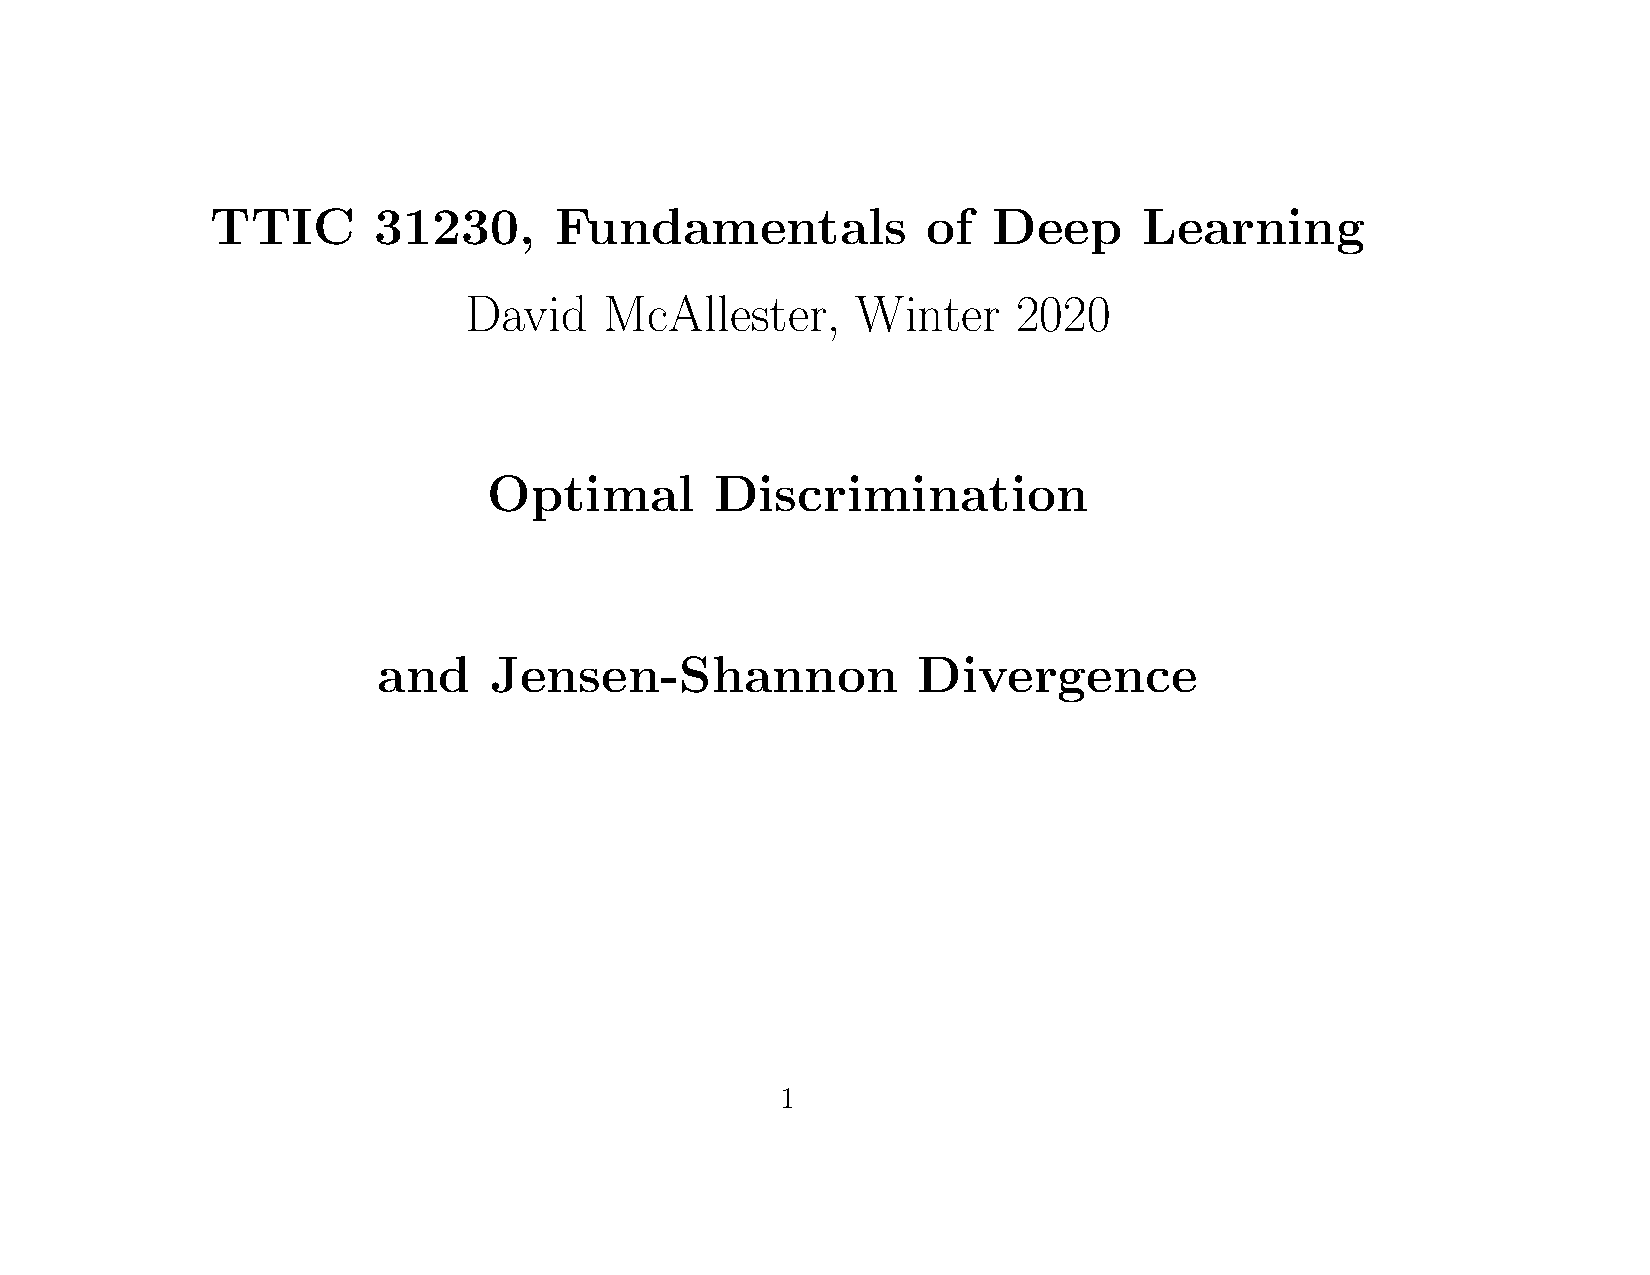
\includegraphics[height = 3.0in]{../images/Jensen}}

\vfill
For $f$ convex (upward curving) we have

\vfill
$$E[f(x)] \geq f(E[x])$$

\slide{Proving $KL(P,Q) \geq 0$}

\begin{eqnarray*}
  KL(P,Q) & = & \expectsub{y \sim P}{- \log \frac{Q(y)}{P(y)}} \\
  \\
  & \geq & - \log \expectsub{y\sim P}{\frac{Q(y)}{P(y)}} \\
  \\
  & = & - \log \sum_y\; P(y) \frac{Q(y)}{P(y)}  \\
  \\
  & = & - \log \sum_y Q(y) \\
  \\
  & = & 0
\end{eqnarray*}

\ignore{
\slideplain{Density Estimation}

Anything that can be done conditionally $P_\Phi(y|x)$ can also be done unconditionally $P_\Phi(y)$.

\vfill
We have unconditional cross-entropy training.

\begin{eqnarray*}
  \Phi^* & = & \argmin_\Phi \;\;E_{y \sim \mathrm{Pop}}  -\log P_\Phi(y)
\end{eqnarray*}

\vfill
This is {\bf distribution modeling} or {\bf density estimation}.

\vfill
Density estimation is sometimes equated with {\bf unsupervised learning}.  A primary example is {\bf language modeling}.

\slide{Unsupervised Learning}

\centerline{\includegraphics[width = 8in]{../images/cake}}


\slide{Unsupervised Learning}

By ``unsupervised learning'' we will mean learning from {\bf massively available} data.  This is not a mathematical definition.

\vfill
{\bf Massive}: images, audio, text, video, click-through data.

\vfill
{\bf Less Massive}: car control data, stereo image pairs, closed captioned video, captioned images.

\vfill
{\bf Big}: Manually annotated images or audio.

\vfill
{\bf Small}: manually annotated text --- parse trees, named entities, semantic roles, coreference, entailment.

\vfill
{\bf Smallest:} Manually annotated text in an obscure language.

\slide{Colorization}

$$\Phi^* = \argmin_\Phi \expectsub{(x,y) \sim \mathrm{Pop}}{-\log P_\Phi(y|x)}$$

\vfill
\centerline{\includegraphics[height=2in]{../images/Colorization}}

\vfill
We have massive data for colorization.

\vfill
Colorization is unsupervised structured labeling.
}

\slide{Summary}

{\color{red} $\Phi^* = \argmin_\Phi\;H(\pop,P_\Phi)$} unconditional

\vfill
{\color{red} $\Phi^* = \argmin_\Phi\;E_{x \sim \pop}\;H(\pop(y|x),P_\Phi(y|x))$} conditional

\vfill
\centerline{
  $\begin{array}{lrcl}
\mathrm{Entropy}: & {\color{red} H(P)} & = & {\color{red} E_{y \sim P}\;-\ln\;P(y)} \\
\\
\mathrm{Cross Entropy:} & {\color{red} H(P,Q)} & = & {\color{red} E_{y \sim P}\;-\ln\;Q(y)} \\
\\
\mathrm{KL\; Divergence:} & {\color{red} KL(P,Q)} & = & {\color{red} H(P,Q) - H(P)} \\
\\
& & = & {\color{red} E_{y \sim P}\;\;\; \ln\;\frac{P(y)}{Q(y)}}
\end{array}$}

\vfill
\centerline{{\color{red} $H(P,Q) \geq H(P),\;\;\;KL(P,Q) \geq 0,\;\;\;\argmin_Q\;H(P,Q) = P$}}


\ignore{
\slide{The Rearrangement Trick}

{\huge
\begin{eqnarray*}
H(P,Q) & \doteq & E_{x \sim P} \;-\ln Q(x) \\
\\
& = & E_{x \sim P}\; -\ln\;\left(P(x)\;\frac{Q(x)}{P(x)}\right) \\
\\
& = & E_{x\sim P}\; \left(-\ln P(x) + \ln \frac{P(x)}{Q(x)}\right) \\
\\
& = & \left(E_{x\sim P}\; -\ln P(x)\right) + \left(E_{x \sim P(x)} \ln \frac{P(x)}{Q(x)}\right) \\
\\
& = & H(P) + KL(P,Q) \\
\\
& \geq & H(P)
\end{eqnarray*}
}
}

\slideplain{Appendix: The Rearrangement Trick}

\begin{eqnarray*}
KL(P,Q) & = & E_{x \sim P} \ln \;\frac{P(x)}{Q(x)} \\
\\
& = & E_{x \sim P} \left[(- \ln Q(x)) - (- \ln P(x))\right] \\
\\
& = & (E_{x\sim P} \;-\ln Q(x)) - (E_{x \sim P}\;-\ln P(x)) \\
\\
& = & H(P,Q) - H(P)
\end{eqnarray*}

\vfill
In general $E_{x \sim P} \;\ln \left(\prod_i A_i\right) = E_{x \sim P} \;\sum_i \ln A_i$ 

\slideplain{Appendix: The Rearrangement Trick}

\begin{eqnarray*}
\mathrm{ELBO} & = & E_{z \sim P_\Psi(z|y)} \ln \;\frac{P_\Phi(z,y)}{P_\Psi(z|y)} \\
\\
\\
 & = & E_{z \sim P_\Psi(z|y)} \ln \;\frac{P_\Phi(z)P_\Phi(y|z)}{P_\Psi(z|y)} \\
\\
\\
 & = & E_{z \sim P_\Psi(z|y)} \ln \;\frac{P_\Phi(y)P_\Phi(z|y)}{P_\Psi(z|y)} \\
\end{eqnarray*}

\vfill
Each of the last two expressions can be grouped three different ways leading to six ways of writing the ELBO.
\slideplain{END}

}
\end{document}
